\chapter{Chemistry's Counting Unit: How Much Is a Mole?}

\begin{kaichang}
Get three things from the kitchen: a bag of rice, a small spoonful of salt, and a cup of water.

First, a simple question: how many grains are in the bag? You probably frown---who has time to count them individually? But ask instead how much the bag weighs, put it on a kitchen scale, and you have an answer in ten seconds.

Now an impossible question: how many water molecules are in the cup? Frowning will not help this time. Even if everyone in the world counted one molecule per second, without eating or sleeping for ten thousand years, they would not count even a fraction of the cup.

Yet chemists can answer that second question, using nothing more than a balance. They have even invented a special counting unit, the mole. Leave yourself one puzzle to guess: which is greater, the number of molecules in a cup of water or the total number of cupfuls the world's oceans can hold? At the end of this chapter, we will check with numbers.
\end{kaichang}

\section{Humans Have Long Known How to Take Counting Shortcuts}

You already count in packages. Eggs come by the dozen: 12 each. Milk comes by the case: 24 cartons. Printer paper comes by the pack: 500 sheets. Nobody says ``give me 0.83 dozen eggs,'' because the point of a dozen is to speed counting and simplify accounts. Such packaging is everywhere: tissues by the pull, stamps by the sheet, batteries by the pack. Filling stations do not count drops at all; they sell fuel by the liter, itself a large package in the liquid world.

Think again about rice. Supermarkets weigh it rather than count grains. Hardware shops are even more direct: buy a box of nails, and the clerk pours them onto a scale. This is \textbf{replacing counting with weighing}, not laziness. It requires just one fact: the average mass of a nail. Divide total mass by individual mass, and the count appears without counting a single nail.

\begin{shiyan}
\textbf{Materials}: a kitchen scale (preferably accurate to 1 gram), a small bowl of rice, paper, and a pen.

\textbf{Procedure}:
\begin{enumerate}[itemsep=1pt]
\item Count 100 grains of rice, put them on the paper, weigh their total mass, and record it (for example, 2.1 grams).
\item Calculate the average mass in grams per grain.
\item Put a handful of rice on the scale and weigh it (say, 37 grams). Before counting, predict the number of grains using the mass per grain you just found, and write it down.
\item Actually count the handful and compare with your prediction.
\end{enumerate}

\textbf{What to observe}: How close was your prediction? How many grains off was it? Where did the error come from---some plump grains and some shriveled ones? Would using 500 grains in step 1 improve the prediction?

\textbf{Safety}: This experiment has no hazards except making your eyes tired from counting rice. Return the rice to its container afterward; do not waste food.
\end{shiyan}

Your reasoning was exactly what chemists use every day: \textbf{treat an individual mass as an exchange rate between total mass and number}. The only difference is that their objects are absurdly smaller than rice grains.

\section{Just How Small Are Atoms?}

How absurdly small? A carbon atom has a mass of about $1.99\times 10^{-23}$ grams. Notice the exponent: after the decimal point come 22 zeros before 199. The world's most sensitive analytical balances can weigh about $10^{-7}$ grams, and already cost as much as a car, yet remain 16 orders of magnitude away from an atom. \textbf{A single atom cannot be weighed, and never can be.}

Consider a grain of salt. It weighs about $6\times 10^{-5}$ grams (60 micrograms), almost too small to see. How many particles does it contain? Salt consists of orderly pairs of sodium and chloride ions (Chapter 18 examines their arrangement). You will soon calculate that this tiny grain contains about $10^{18}$ ion pairs---one quintillion pairs. Count three per second without stopping, day or night, and you would need more than ten billion years, longer than the age of the universe.

Water molecules are more astonishing still. How many are in a 200-gram cup? Put down an outline of the answer now: about $7\times 10^{24}$---seven hundred sextillion. With everyone on Earth counting one per second, it would take thirty thousand years.

Consider smallness from another angle. Visible light's wavelength is thousands of times an atom's diameter. Atoms are smaller than light's ``ripples,'' so however perfectly a microscope lens is polished, light bends around atoms as sea waves bend around tiny stones. Atoms are not merely unseen so far; seeing them with light is impossible in principle. Invisible, uncountable, and individually unweighable: these three difficulties force chemists down the same path.

Chemists therefore face a dead end. Reactions occur particle by particle---two hydrogen molecules to one oxygen molecule, exactly---yet particles cannot be counted or individually weighed. What can be done? The rice experiment gives a clue: \textbf{weigh instead of counting; all we need is an enormous exchange rate}. That exchange rate is this chapter's main character.

\section{Carbon Atoms as Weights: Relative Atomic Mass}

To bridge weighing and counting, we first need a weight for each kind of atom. Actual atomic masses, however, are unwieldy numbers such as $10^{-23}$ grams. Chemists therefore changed their approach: \textbf{compare relative weights instead of absolute weights}, choosing one atom as a standard weight against which to compare others.

They chose carbon-12, the most common carbon atom, with 6 protons and 6 neutrons in its nucleus (Chapter 7 explains isotopes). By definition, its relative mass is \textbf{exactly 12}. Compared with it, hydrogen has a relative mass of about 1, oxygen about 16, and iron about 56. These are \textbf{relative atomic masses}, printed in the periodic table's boxes.

Why go to this trouble? The clever part comes next. One carbon-12 atom has an actual mass of $1.99\times 10^{-23}$ grams. How many together weigh exactly 12 grams? Divide:
\[
\frac{12}{1.99\times 10^{-23}}\approx 6.02\times 10^{23}
\]
The answer is about $6.02\times 10^{23}$. This number's status in chemistry rivals that of pi in geometry. Its name is the \textbf{Avogadro constant}, symbol $N_{\mathrm{A}}$. Since 2019, the International System of Units has fixed it at the exact value:
\[
N_{\mathrm{A}}=6.02214076\times 10^{23}\ \ud{}{mol^{-1}}
\]
(The final $\mathrm{mol^{-1}}$ means ``per mole,'' which we will explain shortly.)

This number gives chemistry its counting unit: \textbf{$6.02\times 10^{23}$ particles make 1 mole}. The mole is the unit of amount of substance, just as ``one'' and ``dozen'' are counting units, except that this package contains 6,020 septillion entities.

\section{A Mole Resembles a Dozen, with Three Differences}

Thinking of a mole as an enlarged dozen is a good start, but three differences matter:

\textbf{First, the magnitudes belong to entirely different worlds.} A dozen is 12; a mole is $6.02\times 10^{23}$. How huge is that? An estimate later will give you a proper shock.

\textbf{Second, a dozen is a convention, while the mole has an exact definition.} Twelve has no special reason behind it; ancient merchants chose it for convenience. But $6.02214076\times 10^{23}$ is an exact value fixed by the SI, anchored to carbon-12 (that anchoring underwent major revision in 2019; see the closing challenge).

\textbf{Third, and most elegantly}, because the Avogadro constant originated from 12 grams of carbon-12, an exceptionally useful property follows automatically: \textbf{the mass in grams of 1 mole of any particle is numerically exactly its relative mass}. Hydrogen atoms have relative mass 1, so a mole weighs 1 gram; oxygen atoms have relative mass 16, so a mole weighs 16 grams. A water molecule's relative mass is $1\times 2+16=18$, so a mole of water molecules weighs 18 grams. For any molecule, add the relative masses of all atoms in its formula to obtain its relative molecular mass, also its grams per mole.

This is the entire secret of counting atoms with a balance. How many molecules are in 200 grams of water? No counting required: $200\div 18\approx 11.1$ moles, multiplied by $6.02\times 10^{23}$ gives about $6.7\times 10^{24}$. The opening impossible question is solved with two lines of division.

\begin{qiaoliang}
Mass, amount of substance, and particle number are three neighboring rooms. Two bridges connect them, each with its own exchange rate:
\[
n=\frac{m}{M}\qquad N=n\times N_{\mathrm{A}}
\]
Here $m$ is mass in grams, $M$ is molar mass in grams per mole (numerically equal to relative mass), $n$ is amount of substance in moles, $N$ is particle number, and $N_{\mathrm{A}}$ is the Avogadro constant.

Practice both directions. How many moles are 9 grams of water? Since $M(\chem{H_2O})=18\ \mathrm{g/mol}$, $n=9\div 18=0.5$ moles, or about $3.01\times 10^{23}$ molecules. Conversely, what do 3 moles of carbon dioxide weigh? With $M(\chem{CO_2})=12+16\times 2=44\ \mathrm{g/mol}$, the answer is $3\times 44=132$ grams.

After every calculation, make two checks. \textbf{Dimensional check}: $m\div M$ has units $\mathrm{g}\div(\mathrm{g/mol})=\mathrm{mol}$. Matching units show that you have not reversed the formula; a monster such as $\mathrm{g^2/mol}$ sends you straight back to find the error. \textbf{Order-of-magnitude check}: ordinary beaker samples weigh grams, so $n$ should lie between $10^{-2}$ and $10^{1}$ moles. A result of $10^{10}$ moles exceeds all the world's water and must be wrong. These two checks take under ten seconds and can catch half the careless errors on an exam.
\end{qiaoliang}

\section{Three Analogies for This Enormous Number}

Written on paper, $6.02\times 10^{23}$ looks ordinary, but it dwarfs everyday intuition. Calibrate your sense of scale with three analogies.

\textbf{Sand.} Suppose a sand grain is a sphere about 0.5 millimeters across, with volume about $6.5\times 10^{-11}$ cubic meters. A mole of sand grains occupies about $4\times 10^{13}$ cubic meters. Spread them evenly over China's roughly 9.6 million square kilometers, and they form a layer about 4 meters deep---an entire country buried one story deep. That is a mole of sand.

\textbf{Time.} How long is a mole of seconds? About $1.9\times 10^{16}$ years. The universe is approximately 13.8 billion, or $1.38\times 10^{10}$, years old. A mole of seconds exceeds a million ages of the universe. Count once per second from the Big Bang until today, and you have not reached even a fraction of a mole.

\textbf{Water.} A mole of water weighs just 18 grams, one swallow: the small side. Yet a 200-gram cup contains about $7\times 10^{24}$ molecules: the large side. The mole stands precisely between them, linking the drinkable, weighable macroscopic world to a particle world numbered in powers of ten in the twenties.

We need an almost hopelessly large package because an individual atom is almost hopelessly small. At $6.02\times 10^{23}$, those two extremes cancel, leaving 18 grams of water, 2 grams of hydrogen, and 56 grams of iron: convenient everyday quantities on a balance. This is no coincidence; it is exactly why the original standard was 12 grams of carbon-12.

\section{Introducing the Symbols, Then Concentration}

So far this chapter has really used just four symbols. Here they are together: amount of substance $n$ (mol), the Avogadro constant $N_{\mathrm{A}}$, molar mass $M$ ($\mathrm{g/mol}$), and particle number $N$. Their relationships fit into one conversion map:

\begin{center}
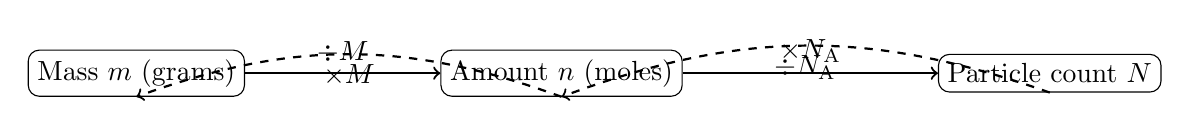
\begin{tikzpicture}
\node[draw,rounded corners] (m) at (0,0) {Mass $m$ (grams)};
\node[draw,rounded corners] (n) at (5.4,0) {Amount $n$ (moles)};
\node[draw,rounded corners] (N) at (11.6,0) {Particle count $N$};
\draw[->,thick] (m) -- (n) node[midway,above] {$\div M$};
\draw[->,thick] (n) -- (N) node[midway,above] {$\times N_{\mathrm{A}}$};
\draw[->,thick,dashed] (n.south) to[bend right=20] node[midway,below] {$\times M$} (m.south);
\draw[->,thick,dashed] (N.south) to[bend right=20] node[midway,below] {$\div N_{\mathrm{A}}$} (n.south);
\end{tikzpicture}
\end{center}

This is simply a human representation: boxes and arrows form a memory aid, not a real picture of matter.

Chemists also ask \textbf{how much stuff occupies how much space or mixture}: concentration. You have seen several versions. The $0.9\%$ label on physiological saline means 0.9 grams of sodium chloride per 100 grams of solution. Air-quality reports use micrograms per cubic meter, mass divided by volume. Chemistry laboratories most often use \textbf{molar concentration}: moles of solute per liter of solution, written $\mathrm{mol/L}$. Physiological saline contains 9 grams of sodium chloride per liter; with $M(\chem{NaCl})\approx 58.5\ \mathrm{g/mol}$, its concentration is about $9\div 58.5\approx 0.154\ \mathrm{mol/L}$.

Concentration has another face: dilution. Put a spoonful of concentrated broth into a pot of water and the flavor immediately weakens. Solute amount stays constant while volume grows, lowering concentration. Laboratories and farms use this principle. A pesticide bottle's ``dilute 1000 times'' means mixing one part preparation with roughly 1000 parts water, reducing concentration to a range that kills pests while minimizing crop damage and excessive soil residues. Drink labels likewise report concentration: cola contains about 10 grams of sugar per 100 milliliters, so a 330-milliliter can contains over 30 grams, about 0.1 mole---close to 20 sugar cubes. Concentration itself is neither good nor bad; dose decides everything. Sodium chloride at $0.9\%$ can be infused into blood vessels, while drinking concentrated brine only dehydrates you.

Reporting concentration in moles helps medicine daily. A fasting blood-glucose result is around $5.6\ \mathrm{mmol/L}$ (mmol means millimole, one thousandth of a mole). An adult has about 5 liters of blood, so total blood glucose is approximately $5.6\times 5=28$ millimoles. With glucose's molar mass of $180\ \mathrm{g/mol}$, that is only about 5 grams---roughly one sugar cube. All your blood glucose amounts to a single cube, and your body must constantly keep it within this narrow range (Chapter 60 on homeostasis revisits this precision control system). Without conversion through moles, you would never recognize $5.6\ \mathrm{mmol/L}$ and ``one sugar cube'' as the same thing.

\section{A Hypothesis Neglected for Half a Century}

\begin{zhengju}
The Avogadro constant bears Avogadro's name, but he neither measured it nor knew its size. In 1811, the Italian physicist proposed that equal volumes of gas at the same temperature and pressure contain equal numbers of molecules. This elegantly explained the volume relationships in gas reactions, but required accepting that atoms of the same element can join into molecules, such as two hydrogen atoms forming one hydrogen molecule. That contradicted leading authorities, and the hypothesis was sidelined for nearly fifty years. Chapter 6 tells the history of atomic theory; here is the key turn. In 1860, chemists from different countries met in Karlsruhe, Germany, arguing even over whether water's formula was HO or \chem{H_2O}. The Italian chemist Cannizzaro distributed a pamphlet using Avogadro's hypothesis to straighten out confused atomic weights. Many young chemists switched sides upon reading it, finally making a shared relative-atomic-mass standard possible.

How was $6.02\times 10^{23}$ itself measured? In 1865, the Austrian Loschmidt used gas kinetic theory to estimate the number of air molecules, producing the first rough account. The truly persuasive work, however, was that of the French physicist Perrin around 1908. He suspended tiny ground gamboge-resin particles in water and watched their Brownian motion individually under a microscope (the ceaseless dance of Chapter 2). Under gravity, he found particles were less numerous higher up, following exactly the same pattern as atmospheric density decreasing with altitude. They behaved like enlarged atoms. From this relationship, he could infer how many water molecules were needed to make them jump so vigorously. He obtained an Avogadro constant between $6\times 10^{23}$ and $7\times 10^{23}$.

This conclusion was decisive because Perrin used several unrelated approaches---Brownian motion, sedimentation equilibrium, and radioactive counting---all leading to the same number. Scientists who firmly denied real atoms, including positivists calling them bookkeeping devices, conceded before this mutual confirmation. Perrin received the 1926 Nobel Prize in Physics. Remember the lesson: whether an invisible thing exists is decided by \textbf{whether independent evidence chains converge on one answer}, not debate. Incidentally, his equipment was remarkably simple: an ordinary microscope, a tall water column, a micrometer scale, and almost endless patience. He counted the heights of thousands of particles individually. Great measurements do not necessarily require expensive instruments, but they do require designs skeptics cannot fault.
\end{zhengju}

\section{The Limits of This Bridge}

Every useful model has boundaries, including the mole.

First, \textbf{the mole requires clearly specified particles of the same kind}. A mole of hydrogen atoms or water molecules makes sense, but ``a mole of sand'' does not: sand mixes grains of different sizes and compositions, with no uniform individual unit. ``A mole of starch'' is similarly awkward. Starch molecules are long chains of hundreds or thousands of glucose units, of varying lengths and without one fixed relative molecular mass (Chapters 43 and 46 revisit such polymers).

Second, \textbf{most relative atomic masses in the periodic table are averages}. Chlorine's 35.5 does not mean a ``number 35.5'' chlorine atom exists. It averages two naturally occurring isotopes in their proportions; an individual chlorine atom has a mass of about 35 or 37. Chapter 7 develops this. For now, remember that averages work perfectly well for calculations without being the weight of any actual atom.

Third, \textbf{the mole counts and does nothing else}. A mole of different substances has the same particle number but different masses and usually volumes. Gases at equal temperature and pressure are an exception---precisely Avogadro's hypothesis, used again in Chapter 4's gas picture and Chapter 26's calculations.

These boundaries do not invalidate the mole. They remind us that each unit serves particular questions. Environmental agencies report air pollution in micrograms per cubic meter, concerned with total mass; toxicologists often convert that to molecules per cubic meter because harm arises from repeated molecular encounters with the body, whose frequency relates directly to particle number. The same pollution, reported two ways, answers different questions. Choosing a counting method is itself part of scientific literacy.

\begin{wuqu}
``A mole of anything weighs the same.'' This is the most common misunderstanding. A mole of hydrogen gas (\chem{H_2}) weighs only 2 grams, while a mole of gold weighs 197 grams, nearly a hundred times more. What the mole guarantees is \textbf{equal particle numbers}: each contains $6.02\times 10^{23}$ basic particles, molecules for hydrogen and atoms for gold. Equal counts do not imply equal masses, any more than a dozen eggs and a dozen watermelons weigh the same. Likewise, the mole is neither a mass unit nor a volume unit; it is a counting unit, and that alone.
\end{wuqu}

\section{Back to the Rice, Salt, and Cup of Water}

Let us keep our opening promise.

The rice bag: you were already using mole-style thinking. Weighing 100 grains gives the average mass per grain; dividing the bag's mass by it gives the count. Chemists do the same, but their individual masses are on the order of $10^{-23}$ grams and their exchange rate on the order of $10^{23}$. \textbf{The Avogadro constant is essentially the reciprocal of the atomic world's mass per rice grain.}

The salt grain: divide its mass, about $6\times 10^{-5}$ grams, by sodium chloride's molar mass, $58.5\ \mathrm{g/mol}$, to get about $10^{-6}$ moles, or approximately $10^{18}$ sodium--chloride ion pairs. Counting would never finish, yet in moles it is merely a millionth of a mole.

The water cup: 200 grams contains about $6.7\times 10^{24}$ molecules. The opening puzzle compared this with the world's oceans, about $1.4\times 10^{24}$ grams of water, yielding only about $7\times 10^{21}$ cups of 200 grams each. \textbf{A cup contains more molecules than all the oceans contain cupfuls---about a thousand times more.} Pour your cup into the sea, mix thoroughly, and scoop out another cup anywhere: on average it contains over a thousand molecules from the original. Your current sip probably includes molecules once drunk by dinosaurs or raised in a toast by the poet Li Bai. This is division, not poetry. In the atomic world, enormous numbers turn eternal cycling into a plain statistical fact.

\section{Why Chemists Must Count}

If weighing is so convenient, why detour through particle counts? Because \textbf{chemical reactions pair particles one-to-one, two-to-one, and so on}. Two hydrogen molecules burn with exactly one oxygen molecule; one carbon atom combines with exactly two oxygen atoms. Recipes are written by number, not mass. In an ammonia plant, one nitrogen molecule needs three hydrogen molecules. Mixing 1 gram of nitrogen with 3 grams of hydrogen would be completely wrong: nitrogen's molar mass is 28 and hydrogen's only 2, so the correct recipe is 28 grams of nitrogen to 6 grams of hydrogen. Without count-based conversion, expensive material remains unused and wasted or contaminates the product. Drug manufacturing and wastewater treatment use exactly the same principle: convert masses to moles before mixing ratios make sense. Hospitals likewise report infusion electrolytes, dialysis-fluid recipes, glucose, and potassium in moles or millimoles because bodily reactions keep accounts by particle number too.

How exactly is this number-based ledger kept? What do chemical-equation coefficients say? Will reactants remain, and how much? These questions are where the mole proves its worth. Chapter 26, ``Chemical Equations Are a Reaction's Ledger,'' will balance the entire account.

\begin{tiaozhan}
On May 20, 2019, the SI underwent major surgery: the Avogadro constant was assigned the \textbf{exact value} $6.02214076\times 10^{23}\ \mathrm{mol^{-1}}$, no longer measured and never revised. This may sound like a game of definitions, but it reversed a dependency. Previously, the kilogram was defined by a platinum--iridium cylinder in Paris, the International Prototype of the Kilogram, while a mole meant the atoms in 12 grams of carbon-12. The mole thus depended on the kilogram. But the prototype could collect dust and wear down; over more than a century, differences of tens of micrograms developed between it and its copies. Defining the world's mass by a changeable metal object could not last. After 2019, the kilogram was defined by fundamental physical constants, the mole by a fixed number of particles, and the cylinder retired honorably. One beautiful engineering contribution used highly pure silicon-28 grown into a single crystal and polished into a nearly perfect one-kilogram sphere. X-rays measured lattice spacing, allowing scientists to count silicon atoms lattice cell by cell---humanity's closest approach to actually counting the atoms. Skipping this section does not interrupt the story, but if you wonder whether definition or measurement has the final say, here is a bridge to physics.
\end{tiaozhan}

\section*{Try It Yourself}

\begin{sikaoti}
\item Copy and complete the conversion map: three boxes for mass, amount of substance, and particle number, joined by four arrow bridges. Beside each bridge, say who collects the toll---which quantity you need for the conversion. This map will help with every later quantitative chapter.
\item Without looking anything up, estimate the number of molecules in a drop of water, about 0.05 grams. Then calculate how many years a supermachine counting one million per second would need to count them all.
\item Which contains more molecules: 4 grams of hydrogen (\chem{H_2}) or 32 grams of oxygen (\chem{O_2})? How many does each contain? (Hint: first find molar masses; compare $n$, not mass.)
\item A student misremembers the formula as $n=M\div m$. Prove it must be wrong using dimensional analysis alone, without inserting numbers.
\item Dissolve 9 grams of sodium chloride (\chem{NaCl}) and add water to a total volume of 1 liter. What is the molar concentration? Compare it with laboratory physiological saline ($0.9\%$). What do you notice?
\item Estimate the mass of a mole of rice grains (one grain is about 0.02 grams), then compare it with annual world grain production, about $3\times 10^{12}$ kilograms. This comparison shows why the Avogadro constant belongs only to the atomic world.
\end{sikaoti}
